\section{Solow model}

\underline{Mechanism of Solow model}

\begin{itemize}
    \item Firms: producing output using capital
    \item Consumers: consume output and save fraction of income $\rightarrow$ future capital $\rightarrow$ produce $\rightarrow$ save
\end{itemize}

\underline{Basic Assumptions}

\begin{itemize}
    \item Discrete time
    \item Closed economy, single good: for consumption and investment
    \item Two actors in the economy: firms and households
          \begin{itemize}
            \item Firms: produce output using capital and Labor
            \item Households: receives labor and capital income,
            and profits from owning the firms(now $=0$); consume and save
          \end{itemize}
    \item Three markets: labor, capital and final goods
\end{itemize}

\subsection{Households(HH)}

\begin{note}
    \ 

    Households do not optimize, which is the main difference to Ramsey model.
\end{note}

Assuming the received income as below:
\[
Y_t = \underset{\text{labor income}}{\underbrace{w(t) L^s(t)}} + \underset{\text{capital income}}{\underbrace{R(t) K^s(t)}} + \underset{profits}{\underbrace{\Pi (t)}}
\]

\underline{Keynesian consumption function}
\[S_t = sY_t \quad C_t = (1-s)Y_t,\]
where $s$ is the saving rate.

\underline{Technology}

Firms produce according to the production function:
\[Y_t = F(K_t, L_t, A_t)\]
where $L$ and $K$ are labor and capital, $A$ is the technology level.

Function $F$ is the \textit{neoclassical production function} with the following properties:
\begin{itemize}
    \item Constant returns to scale:
            \[F(\lambda K, \lambda L, A) = \lambda F(K, L, A)\]
    \item Diminishing marginal products for both $K$ and $L$
            \[\frac{\partial F}{\partial K} > 0, \quad \frac{\partial F^2}{\partial^2 K}<0\]
    \item Inada conditions(likewise for both $L$ and $K$)
            \[\lim_{K \to 0} \frac{\partial F}{\partial K} = \infty, \quad \lim_{K \to \infty} \frac{\partial F}{\partial K} = 0\]
\end{itemize}

\begin{assumption}
    \ 

    \begin{itemize}
        \item All markets are perfectly competitive;
        \item Labor market clearing: $L^s(t) = L^d(t) \equiv L_t$;
        \item Capital market clearing: $K^s(t) = K^d(t) \equiv K_t$;
        \item Goods market clearing: $Y_t = C_t + I_t$: total supply equals to consumption plus investment.
    \end{itemize}
\end{assumption}

\begin{theorem}[Law of motion of capital]\label{Fundamental Law of Motion}
    \[K_{t+1} = (1-\delta)K_t + I_t\]
    where $\delta$ is the depreciation rate, $K(0)$ is the initial capital endowment.    
\end{theorem}

\subsection{Firms}

The firm's problem is to maximize profits:
\[\max_{K, L} \Pi(t) = F(K, L, A_t) - w(t)L_t - R(t)K_t.\]

Taking the FOCs:
\[\frac{\partial F}{\partial K} = R(t), \quad \frac{\partial F}{\partial L} = w(t).\]
Also, we know that 
\[F(K, L, A) = \frac{\partial F}{\partial K} + \frac{\partial F}{\partial L}L,\]
so we can get:
\[\Pi = F(K, L, A) - R(t)K - w(t)L = 0.\]

The equilibrium of the Solow Model is:
\begin{itemize}
    \item $K_{t+1} = (1-\delta)K_t + S_t$
    \item $C_t = (1-s)Y_t$
    \item $S_t = sY_t$
\end{itemize}

From the Fundamental Law of Motion \ref{Fundamental Law of Motion}, we can get:
\begin{align}
    K_{t+1} &= (1-\delta)K_t + S_t\\
    &= (1-\delta)K_t + sY_t\\
    &= (1-\delta)K_t + sF(K_t, L_t, A_t)\\
\end{align}

\subsection{The canonical Solow Model}

\begin{assumption}
    \ 

    \begin{itemize}
        \item No populaiton growth $L_t = L$
        \item No technological progress $A_t = A$
    \end{itemize}
\end{assumption}
Then, we transform the equation (3) into per-capita terms:
\begin{align}
    k_{t+1} &= \frac{K_{t+1}}{L_{t+1}} = (1-\delta) \frac{K_t}{L_t} + s\frac{F(K_t), L, A}{L_t}\\
    &= (1-\delta)k_t + sF(k_t, 1, A) \\
    &= (1-\delta)k_t + sf(k_t)
\end{align}
where $k_t = \frac{K_t}{L_t}$ is the capital per capita, $f(k_t) = F(K_t/L_t, 1, A)$.

Similarly, we have the output per capita:
\[y(t) = \frac{Y_t}{L_t} = \frac{F(K_t, L, A)}{L} = f(k_t),\]
the rate of capital:
\[R(t) = F_K(K_t, L, A) = f^{\prime}(k_t),\]
and the wage rate:
\[w(t) = F_L(K_t, L, A) = f(k_t) - k_tf^{\prime}(k_t).\]

\subsection{Dynamic evolution of the economy}

Characterize everything in term sof uniqeu state variables $k_t$:
\[k_{t+1} = (1 - \delta)k_t + sf(k_t)\]
with $k(0)$ given.

\begin{definition}[Steady state]
    \

    A steady state is a state of the economy where all variables are constant over time.

    The concept corresponding to the steady state in the basic model is the \textit{balanced 
    growth path} (some researchers still prefer to use the name “steady state” for the balanced 
    growth path, because the normalized variables are “steady” also in this case).
\end{definition}

\underline{Steady state of the Solow Model}

There are actually two steady states in the Solow Model:
\begin{itemize}
    \item The trivial steady state: $k^* = 0$
    \item The non-trivial steady state: $k^* > 0$
\end{itemize}
But we can actually ignore the one at $k_t = 0$.

\begin{figure}[!htbp]
    \centering
    \begin{tikzpicture}[>=stealth]
        % Draw axes
        \draw[->] (0,0) -- (4,0) node[right] {\footnotesize $k_t$};
        \draw[->] (0,0) -- (0,4) node[left] {\footnotesize $k_{t+1}$};
        
        % Draw the 45-degree line
        \draw[dashed] (0,0) -- (3.6,3.6) node[right] {\footnotesize 45$^\circ$};
        
        % Draw the curve
        \draw[thick,domain=0:3.7,smooth,variable=\x] plot ({\x},{4*\x/(1+\x)}) node[below right] {\footnotesize $sf(k_t) + (1-\delta)k_t$};
        
        % Mark k* on both axes
        \draw[dashed] (3,0) -- (3,3) -- (0,3);
        \node[below] at (3,0) {\footnotesize $k^*$};
        \node[left] at (0,3) {\footnotesize $k^*$};
    \end{tikzpicture}
    \caption{Steady state of Solow Model}
\end{figure}

\underline{Steady state anlaysis}

At the steady-state, $k^*$ satisfies:
\[\underset{\text{Depreciation}}{\underbrace{\delta k^*}} = \underset{\text{Investment}}{\underbrace{sf(k^*)}} \]
which means that the investment equals to the depreciation.

$k^*$ defined by:
\[\frac{f(k^*)}{k^*} = \frac{\delta}{s}.\]

\underline{A different representation}
In the steady state, the amount of actual investment is exactly such that it compensates for depreciation.

\begin{figure}[!htbp]
    \centering
    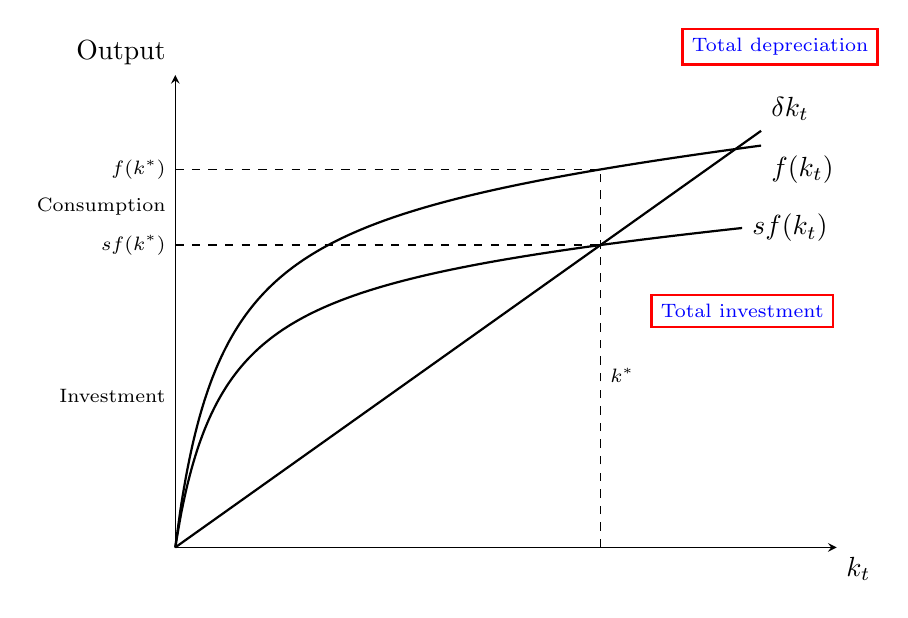
\begin{tikzpicture}[>=stealth, scale=1.2]

        % Draw axes
        \draw[->] (0,0) -- (7,0) node[below right] {$k_t$};
        \draw[->] (0,0) -- (0,5) node[above left] {Output};
        
        % Draw the curves
        \draw[thick,domain=0:6.2,samples=100,smooth,variable=\x] plot ({\x},{4*\x/(0.5+\x) + 0.4/4.5*\x}) node[below right] {$f(k_t)$};
        \draw[thick,domain=0:6,samples=100,smooth,variable=\x] plot ({\x},{3.2*\x/(0.5+\x) + 0.32/4.5*\x}) node[right] {$sf(k_t)$};
        \draw[thick,domain=0:6.2] plot ({\x},{3.2/4.5*\x}) node[above right] {$\delta k_t$};
        
        % Dashed lines for steady state
        \draw[dashed] (4.5,0) -- (4.5,4) node[pos=0.5,below right] {\scriptsize $k^*$};
        \draw[dashed] (0,4) -- (4.5,4);
        \draw[dashed] (0,3.2) -- (4.5,3.2);
        
        % Labels for key points
        \node[left] at (0,4) {\scriptsize $f(k^*)$};
        \node[left] at (0,3.2) {\scriptsize $sf(k^*)$};
        
        % Annotations with boxes
        \node[draw=red, thick, fill=white] at (6.4,5.3) {\scriptsize \textcolor{blue}{Total depreciation}};
        \node[draw=red, thick, fill=white] at (6,2.5) {\scriptsize \textcolor{blue}{Total investment}};
        
        % Investment and consumption text
        \node at (0,1.6) [left] {\scriptsize Investment};
        \node at (0,3.6) [left] {\scriptsize Consumption};
    \end{tikzpicture}
    \caption{Alternative representation of Solow Model SS}
\end{figure}

\underline{Comparative statics}

At the steady state, $k^*$ satisfies:
\[\frac{f(k^*(s, \delta, A), A)}{k^*(s, \delta, A)} = \frac{\delta}{s}\]
while the differentian yields the comparative statics:
\begin{align*}
    \frac{\partial k^*(s, \delta, A)}{\partial \delta} &<0\\
    \frac{\partial k^*(s, \delta, A)}{\partial s} &>0\\
    \frac{\partial k^*(s, \delta, A)}{\partial A} &>0
\end{align*}
The higher productivity A has the 'multiplier' effect on the output directly via $k^*$.

At the steady state, the consumption per capita is:
\[c^* = c(k^*(s, \delta, A)) = (1-s) f(k^*(s, \delta, A)).\]
$s$ has two opposing effects:
\begin{itemize}
    \item Higher $s$ leads to higher $k^*$, which leads to higher $y^*$;
    \item Higher $s$ leads to lower $1-s$, which leads to lower fraction of output consumed.
\end{itemize}

Let $\hat{s}$ be the savings rate that maximizes consumption, i.e.
\[\hat{s} = \arg \max_s (1-s)f(k^*(s, \delta, A)) = \arg \max_{s} \left\{f(k^*(s, \delta, A)) - \delta k^*(s, \delta, A)\right\}.\]
Hence $\hat{s}$ is implicitly defined by:
\[f^{\prime} (k^*(\hat{s}, \delta)) = \delta. \]

\begin{definition}[Golden Rule]\label{Golden Rule}
    \

    The Golden Rule is the savings rate that maximizes consumption in the steady state,
    which is $\hat{s}$ in our model. And, we have $k^{gold} = f'^{-1}(\delta)$ as
    the golden rule capital stock.

    \begin{note}
        \ 

        \begin{itemize}
            \item Savings are excessive if depreciation is higher than the marginal
            product of capital;
            \item By saving less, consumption go up;
            \item The economy is dynamically inefficient if $k>k^{gold}$.
        \end{itemize}
    \end{note}
\end{definition}

\subsection{Growth in the Solow Model}

Dynamics is fully determined by the evolution of capital:
\begin{align*}
    g_k(t) &= \frac{k_{t+1} - k_t}{k_t}\\
    &= \frac{(1-\delta)k_t + sf(k_t) - k_t}{k_t}\\
    &= s\frac{f(k_t)}{k_t}-\delta\\
    &= g_k(k_t)
\end{align*}
So, in the long run, the growth rate of capital is constant and equal to $\frac{sf(k^*)}{k^*} - \delta$.
As long as $k_t<k^*$, the growth rate of capital is positive, and vice versa.

\subsection{The Growing Economy}

Now we extend the model to the situation where $A_t$ and $L_t$ grow over time. 
In the previous section, the long-run outcome was the steady state where there is no growth.
This extension is necessary for addressing the facts related to the growth issues described in later chapters.

We assume that the aggregate production function takes the form of
\[
Y_t = F(K_t, A_t L_t).
\]
There are two changes from the basic model: 
first, we allow the labor input (population times hours worked per person) $L_t$ to grow over time. 
Second, and more importantly, we allow for technological progress. 
In this production function, the variable representing the technology level, $A_t$, 
is multiplied by labor input $L_t$. 
Technological progress thus takes a form of improving the labor input, 
and $A_t L_t$ is often referred to as the total number of efficiency units of labor (or effective labor). 

This form of technological progress is labor-augmenting; it was introduced in the previous chapter. 
As was also asserted there, Uzawa (1961) proved that labor-augmenting technical change is the only form of technical progress that is consistent with exact balanced growth, 
that is, the growth path where aggregate variables such as output and capital grow at a constant rate. 
% Uzawa's theorem is formally stated and proved in Appendix 3.A.

We assume that the (net) growth rate of $A_t$ is $\frac{\dot{A_t}}{A_t} = g$ and that the growth rate of $L_t$ is $\frac{\dot{L_t}}{L_t} = n$. The same manipulations of equations as in the basic model yield
\[
K_{t+1} = (1 - \delta)K_t + sF(K_t, A_t L_t).
\]
The dynamic equation for capital in continuous time is
\[
\dot{K_t} = sF(K_t, A_t L_t) - \delta K_t.
\]
Let us define the efficient unit of capital $k_t$ by
\[
k_t = \frac{K_t}{A_t L_t}.
\]
and take the log derivative w.r.t. time,
\[
\frac{\dot{k_t}}{k_t} = \frac{\dot{K_t}}{K_t} - \frac{\dot{A_t}}{A_t} - \frac{\dot{L_t}}{L_t} = \frac{\dot{k_t}}{k_t} - g - n.
\]
Output per efficiency unit of labor is:
\[
\hat{y_t} = \frac{Y_t}{A_t L_t} = F(k_t, 1) = f(k_t).
\]
Here, $f(k_t) = F(k_t, 1)$ as in the basic model. Hence, the above equation can be written as:
\begin{align*}
    \frac{\dot{k_t}}{k_t} &= \frac{sF(K_t, A_t L_t) - \delta K_t}{K_t} - g - n\\
    &= \frac{sF(K_t, A_t L_t)}{K_t} - (\delta + g + n) \\
    &= \frac{sf(k_t)}{k_t} - (\delta + g + n).
\end{align*}
Therefore, we can get the dynamic of efficient capital $k_t$ as
\[
\dot{k_t} = sf(k_t) - (\delta + g + n)k_t.
\]
After the capital stock $K_t$ is normalized by $A_t L_t$, 
we thus obtain a very similar difference equation as the fundamental equation in the basic model,
with effective depreciation rate $\delta + g + n$.

In this case, upon entering a balanced growth path, 
the rate of per capita output growth depends uniquely on the rate of technological progress $g$.

\subsection{Growth effects of changes in the savings rate}
Consider the consumption path $c^*$ per unit of effective labor, especially in the context of returning to equilibrium and whether the consumption level per unit of effective labor will be above, below, or equal to the level during the previous equilibrium.

This analysis depends on a proposition: an increase in the savings rate persistently raises the average capital stock per unit of effective labor, as well as savings and output levels. The question then arises whether it also implies an increase or decrease in the consumption level per unit of effective labor. Under what conditions does consumption per unit of effective labor reach its optimum?

\underline{Impact of Savings Rate Changes on Optimal Consumption per Unit of Effective Labor}

The formula:
\begin{align*}
    c^* &= f(k^*) - s f(k^*) = f(k^*) - (n + g + \delta) k^* \\
    \frac{\partial c^*}{\partial s} &= \left[f'(k^*(s, n, g, \delta)) - (n + g + \delta) \right] \frac{\partial k^*}{\partial s}
\end{align*}
reveals that whether an increase in the savings rate leads to a long-term rise in consumption per unit of effective labor 
depends on the comparison between the marginal product of capital at the steady-state per capita capital stock and the slope of the investment schedule. 

This formula assists in addressing the query raised in the consumption path analysis diagram.

When the long-term steady-state capital stock per unit of effective labor satisfies the condition that $f^{\prime} (k^*) = n + g + \delta$, 
\textit{the capital stock per unit of effective labor} reaches the golden-rule(\ref{Golden Rule}) level, 
and \textit{the consumption per unit of effective labor is optimal}.

\underline{Impact of Changes in the Savings Rate on the Output of Steady-State Efficient Labor, Capital Stocks}

A rise in the savings rate can lead to a change in the amount of capital in steady state efficient labor:
\begin{align*}
s f(k^*(s,n,g,\delta)) &= (n + g + \delta) k^*(s,n,g,\delta) \\
f(k^*(s,n,g,\delta)) + s f'(k^*) \frac{\partial k^*}{\partial s} &= (n + g + \delta) \frac{\partial k^*}{\partial s} \\
\frac{\partial k^*}{\partial s} = \frac{f(k^*)}{(n + g + \delta) - s f'(k^*)} &> 0
\end{align*}

The sensitivity of the steady state capital per effective labor to the savings rate is crucial. Under the condition that the derivative \(s'f(k^*)\) is smaller than \((n + g + \delta)\), implying that the change in the steady state capital stock \(dk^*/ds < 0\), an increase in the savings rate will initially reduce the consumption per effective worker until new equilibrium is achieved.

Further, the change in production per effective labor \(y^*\) with respect to the savings rate is given by:
\begin{align*}
\frac{\partial y^*}{\partial s} &= f'(k^*) \frac{\partial k^*(s, n, g, \delta)}{\partial s} = \frac{f^{\prime}(k^*) f(k^*)}{(n + g + \delta) - sf^{\prime}(k^*)} > 0
\end{align*}

Finally, the response of production per effective labor to changes in the savings rate can be expressed as:
\begin{align*}
    \frac{s}{y^*} \frac{\partial y^*}{\partial s} &= \frac{s}{f(k^*)} \frac{f^{\prime}(k^*) f(k^*)}{(n + g + \delta) - s f^{\prime}(k^*)} \\
    &= \frac{(n+g+\delta) k^* f^{\prime}(k^*)}{f(k^*) \left[(n+g+\delta) - (n+g+\delta) k^* f^{\prime}(k^*) / f(k^*)\right]} \\
    &= \frac{k^* f^{\prime}(k^*) / f(k^*)}{1 - k^* f^{\prime}(k^*) / f(k^*)} \\ 
    &= \frac{\alpha_k(k^*)}{1 - \alpha_k(k^*)}
    \end{align*}
where \( \alpha_k(k^*) \) represents the output elasticity of capital at the steady state. 
This equation helps in determining whether the increase in the savings rate will eventually 
increase the consumption level per unit of effective labor in the long run.

\begin{summary}
    \

    \begin{itemize}
        \item Baseline Model: 
            \begin{itemize}
                \item No long-run growth, i.e. capital accumulation alone does not make
                the economy grow in the long run
                \item Conditional convergence: if countries have the same parameters $s, \delta, A$
                and the same production function $F$, they will converge to the same
                steady state. Countries further from the steady state will grow faster.
                \item Crucial mechanism: decreasing marginal product to capital
            \end{itemize}
        \item Extended Model:
            \begin{itemize}
                \item Long-run growth poible if productivity grows: $g>0$;
                \item Consistant with Kaldor facts if $g>0$;
            \end{itemize}
        But $s$ and $g$ are exogenous.
    \end{itemize}
\end{summary}

\section{Development Accounting}
Development accounting asks whether the factors of production can explain income levels(See Caselli 2005\cite{caselli2005accounting}).

Assuming the production function is Cobb-Douglas in physical and human capital(more general than labor):
\begin{align*}
    Y_j &= A_j K_j^{\alpha} (L_j h_j)^{1-\alpha}\\
    y_j &= F(k_j, h_j, A_j) = A_j k_j^{\alpha} h_j^{1-\alpha} = A_j y_j^{KH} 
\end{align*}
Casselli(2005) use the following method to measure success:
\[\text{success} = \frac{\var\left[ \log(y_j^{KH} )\right] }{\var\left[\log(y_j)\right]}.\]
Then, if all countries had the same technology $A_j$, then the success would be 1.

How to measure human capital? Not directly observable. But: can
see distribution of schooling in the population, and can see
individual's wage and schooling.

From the production function
\[Y_j = K_j^{\alpha} (A_j H_j)^{1-\alpha}\]
we can calibrate the relative productivity differences relative to the US as
\[\frac{A_j}{A_{US}} = \left(\frac{Y_j}{Y_{US}}\right)^{\frac{1}{1-\alpha}} \left(\frac{K_{US}}{K_{j}}\right)^{\frac{\alpha}{1-\alpha}} \frac{H_{US}}{H_j}.\]
